\documentclass[a4paper, 11pt, onecolumn, openany, titlepage]{report}
\usepackage[utf8]{inputenc}
\usepackage{enumitem}
\usepackage{filecontents}
\usepackage[T1]{fontenc}
\usepackage{url}
\usepackage{breakcites}
\usepackage{graphicx}
\graphicspath{{qualitative-results/}{quantitative-results/}}
\usepackage{caption}
\usepackage{subcaption}
\usepackage{titlesec}
\usepackage{tabularx}
\usepackage{afterpage}
\usepackage{geometry}
\usepackage{hyperref}
\usepackage[rightcaption]{sidecap}
\usepackage[usenames, dvipsnames]{xcolor}
\usepackage[nottoc]{tocbibind}
\usepackage[section]{placeins}
\usepackage{float}
\usepackage[parfill]{parskip}
\usepackage{amsmath}
\usepackage{amsthm}
\usepackage{algorithm}
\usepackage{algpseudocode}
\usepackage{amsfonts}
\usepackage{amssymb}
\usepackage{bbm}
\usepackage{float}

\geometry{a4paper, headsep=1.0cm, footskip=1cm, lmargin=3cm, rmargin=3cm, tmargin=3cm, bmargin=3cm}
\hypersetup{colorlinks, citecolor=NavyBlue, filecolor=NavyBlue, linkcolor=NavyBlue, urlcolor=NavyBlue}

\titleformat{\chapter}[block]{\normalfont\huge\bfseries}{\thechapter.}{5pt}{\huge}
\titlespacing*{\chapter}{0pt}{-19pt}{25pt}
\titleformat{\section}[block]{\normalfont\Large\bfseries}{\thesection.}{5pt}{\Large}

\newcommand\blankpage{\null\thispagestyle{empty}\newpage}
\newcommand\numberedchapter[1]{\setlength\topskip{3cm}\chapter{#1}\setlength\topskip{0cm}}
\newcommand\unnumberedchapter[1]{\setlength\topskip{3cm}\chapter*{#1}\setlength\topskip{0cm}}

\newtheoremstyle{default_theorem_style}
  {1em plus .2em minus .1em}%   Space above
  {1em plus .2em minus .1em}%   Space below
  {\slshape}%  Body font
  {}%          Indent amount (empty = no indent, \parindent = para indent)
  {\bfseries}% Thm head font
  {.}%         Punctuation after thm head
  {0.5em}%     Space after thm head: " " = normal interword space;
     %         \newline = linebreak
  {}%          Thm head spec (can be left empty, meaning `normal')


\theoremstyle{default_theorem_style}\newtheorem{theorem}{Theorem}
\theoremstyle{default_theorem_style}\newtheorem{definition}{Definition}

\begin{document}
\setlength\topskip{3cm}
\newpage
\thispagestyle{empty}
\begin{center}
\textbf{\large Uniwersytet Wrocławski\\
Wydział Matematyki i Informatyki\\
Instytut Matematyczny}\\
\vspace{4cm}
\textbf{\textit{\large Dawid Wegner}\\
\vspace{0.5cm}
{\Large Efektywne odszumianie obrazów przy użyciu algorytmu Metropolis-Hastings}}\\
\end{center}
\vspace{3cm}
{\large \hspace*{6.5cm}Praca licencjacka\\
\hspace*{6.5cm}napisana pod kierunkiem\\
\hspace*{6.5cm}dr hab. Pawła Lorka}\\
\vfill
\begin{center}
{\large Wrocław 2021}\\
\end{center}
\setlength\topskip{0cm}
\afterpage{\blankpage}

{\hypersetup{linkcolor=black}
\setlength\topskip{3cm}
\tableofcontents
\setlength\topskip{0cm}
}

\unnumberedchapter{Introduction}
\addcontentsline{toc}{chapter}{Introduction}

TODO

\numberedchapter{Markov Chains}

In this chapter we will formally define the notion of Markov Chain and list its basic properties.\ Particularly,
we will characterise a stationary distribution and reversible Markov Chains.\ These tools are necessary to understand
the theory behind Markov Chain Monte Carlo methods that are discussed in \textit{Chapter} \ref{chapter:mcmc}.

\section{Basic properties}

Formally, a Markov Chain is a stochastic process in which the probability of the next event depends only on the current
state.\ Intuitively, we can think of such process as a directed graph with loops.\ An example of a Markov Chain that
describes weather conditions is shown in Figure \ref{fig:markov_chain}.\ In this case, our state space contains three
elements: $\{Sun,\ Cloudy,\ Rain\}$.\ Each directed edge represents the probability of transitioning from a state
$X_{n}$ to a state $X_{n + 1}$.\ In the example presented in Figure \ref{fig:markov_chain}, the probability that the
weather will be \textit{rainy} in the day $X_{n + 1}$, conditioned on the fact that it was \textit{cloudy} in the
day $X_n$, is equal to $0.5$.\ Note that the described process carries an underlying assumption that the weather in
the next day depends only on the weather in the present day.

\begin{figure}[H]
\centering
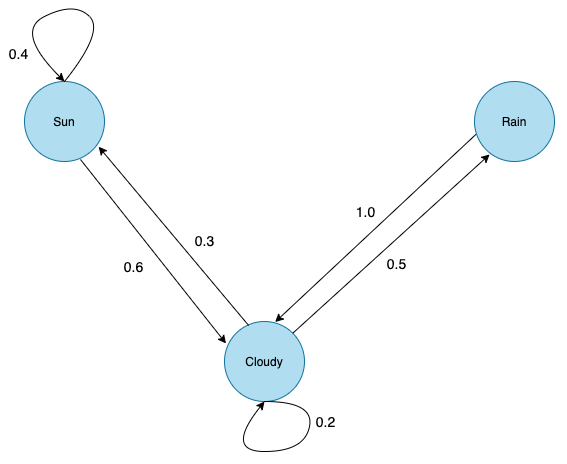
\includegraphics[scale=0.4]{markov_chain}
\caption{An example of a Markov Chain describing weather conditions.}
\label{fig:markov_chain}
\end{figure}

While a graph representation of a Markov Chain is useful, in most cases it's convenient to think of it as a matrix.
Formally, let us define an element $0 \leq P_{ij} \leq 1$ of a matrix $P$ as the probability of
transitioning from the state $i$ to the state $j$.\ As the $i$-th row of such matrix defines probabilities of
transitioning from the $i$-th  state to all other states, the equality $\sum_{j = 1}^{n} P_{ij} = 1$ holds.\ A
matrix with the above-mentioned properties is called a \textit{stochastic} matrix.\ In the next sections, we will think
of a Markov Chain in this way.

\begin{definition}
A vector $\mu^{(0)} = (\mu^{(0)}_1, \mu^{(0)}_2, \dots, \mu^{(0)}_n)$ such that $\sum_{i=1}^{n} \mu^{(0)}_i = 1$
is called an \textit{initial state} of a Markov Chain.\ It defines an initial distribution across the state space.

\end{definition}

The Markov Chain process is fully characterized by its transition matrix $P$ and an initial state $\mu^{(0)}$.\ In
particular, the distribution of a Markov Chain in the $k$-th step can be uniquely determined i.e.\ the equality
$\mu^{(k)} = \mu^{(0)}P^k$ holds.\ Although a Markov Chain can contain infinitely many states, we only consider
the ones with a finite number of states.\ In particular, some theorems presented in the next sections
are not true without this assumption.\newline

\section{Stationary distribution}

In this section we will formalize the notion of stationary distribution and explore its properties.\ Furthermore,
we will provide sufficient conditions to guarantee that a Markov Chain has a unique stationary distribution.

\begin{definition}
A vector $\pi = (\pi_1, \pi_2, \dots, \pi_n)$ is called a \textit{stationary} distribution if and only if $\pi P = \pi$,
where $P$ denotes a transition matrix of a Markov Chain.
\end{definition}

One can convince yourself that a Markov Chain can have multiple stationary distributions.\ An example of such Markov
Chain is when $P = Id$, which implies that any probability distribution is stationary.\ In the remaining part of this
section we will characterise a family of Markov Chains with a unique stationary distribution.

\begin{definition}
A Markov Chain with a transition matrix $P$ is called \textit{irreducible} if and only if for each pair of the source
state $i$ and the destination state $j$, it's possible to transition from $i$ to $j$ in a finite time i.e.\ there
exists $k$ such that $(P^k)_{ij} > 0$.
\end{definition}

\begin{definition}
A period of the $i$-th state is defined as $p(i) = gcd(\{n \geq 1 : (P^n)_{ii} > 0\}$.\ A state is called
\textit{aperiodic} if $p(i) = 1$.\ A Markov Chain is called aperiodic if all of its states are aperiodic.
\end{definition}

A Markov Chain that respects the two above-mentioned properties is called an \textit{ergodic} Markov
Chain.\ Interestingly, ergodic Markov Chains have many useful properties that leads to sophisticated algorithms.

\begin{theorem}\label{thm:one_stationary}
For any ergodic Markov Chain, there exists exactly one stationary distribution $\pi$.
\end{theorem}

\begin{theorem}\label{thm:converges_to_stationary}
Let $\mu^{(0)}$ be an arbitrary initial state of any ergodic Markov Chain.\ Let
$d_{TV}(\mu^{(n)}, \pi) = \frac{1}{2} \sum_{i = 1}^{k} |\mu_i^{(n)} - \pi_i|$ denote a distance between a
distribution of possible states in the $n$-th step and a stationary distribution of the defined Markov Chain.\ Then,
the equality $\lim_{n \to \infty} d_{TV}(\mu^{(n)}, \pi) = 0$ holds.
\end{theorem}

The proofs of \textit{Theorem} \ref{thm:one_stationary} and \textit{Theorem} \ref{thm:converges_to_stationary} can
be found in \cite{markov_chains_book}.\ From the practical point of view, the presented theorems imply that an
ergodic Markov Chain always converges to its stationary distribution, regardless of the initial
distribution.\ Note that the presented theorems do not guarantee any convergence speed.

\section{Reversible Markov Chains}

Reversible Markov Chains show up in many different areas e.g.\ they are the main building block for the Markov
Chain Monte Carlo methods.\ Formally, the reversed process is defined as $\tilde{X_t} = X_{T - t}$.\ Intuitively,
$\tilde{X}$ represents a Markov chain that is reversed in a time.

\begin{definition}
A probability distribution $\tilde{\pi}$ is said to be \textit{reversible} for a Markov Chain with a transition
matrix $P$ if and only if for any $i,j$ it holds $\tilde{\pi_i} P_{ij} = \tilde{\pi_j} P_{ji}$.\ A Markov Chain
is called a $reversible$ chain iff $\tilde{X_t} = X_t$ i.e. the reversed process is the same as the forward process.
\end{definition}

\begin{theorem}\label{reversible_chain}
A Markov Chain with a stationary distribution $\pi$ is reversible if and only if for any $i, j$ the equality
$\pi_i P_{ij} = \pi_j P_{ji}$ holds.
\end{theorem}

\textit{Theorem} \ref{reversible_chain} has many useful implications.\ First of all, in order to determine whether
a distribution is reversible, it suffices to check if it exists a probability measure $\tilde{\pi}$ such that
for any $i, j$ the equality $\tilde{\pi_i} P_{ij} = \tilde{\pi_j} P_{ji}$ holds.\ What is more, in case we find such
$\tilde{\pi}$, it follows that $\pi = \tilde{\pi}$ i.e.\ the probability measure that we found is a stationary
distribution.\ As a result, this equation gives us a powerful tool for finding a stationary distribution.

\numberedchapter{Markov Chain Monte Carlo methods}\label{chapter:mcmc}

Consider a problem of sampling a random permutation from the set of $100$ elements.\ One can show that such space
contains $100!$ elements, implying that putting all permutations in the memory of a computer is not feasible.\ While
there exist algorithms for sampling permutations from a uniform distribution, the problem becomes harder in the case of
a skewed distribution.\ For instance, let our target distribution be defined based on positions of permutation's
elements e.g.\ $d(x) = \prod_{i = 1}^{n} e^{i \cdot x_i}$, where $x_i$ denotes the $i$-th element of the
permutation.\ While the problem of sampling from such distribution can not be tackled using any trivial algorithm,
it's possible to simulate the sampling process with Markov Chains.\newline

In this chapter, we will show how to deal with a situation in which we have a large state space and our task is to
sample an element from this space effectively.\ We will leverage the theory presented in the previous section to
show how to construct a Markov Chain with a stationary distribution equal to the target distribution we want to
sample from.

\section{Metropolis–Hastings algorithm}

Let us denote the target distribution we want to sample from as $\tilde{\pi}$.\ Notice that in order to produce samples
from $\tilde{\pi}$ one may construct a Markov Chain $X$ with a transition matrix $P$ and a stationary distribution
$\pi = \tilde{\pi}$.\ As a result, it suffices to simulate $X$ until we reach the stationary distribution.\ Assuming
that $X$ is ergodic, it can start in any initial state and based on \textit{Theorem} \ref{thm:converges_to_stationary}
it is guaranteed to converge to $\pi$.\ As one of our assumptions says that the space of states is very large,
constructing such Markov Chain explicitly does not solve our problem.\ Nevertheless, we can simulate such Markov Chain
with the Metropolis-Hastings algorithm.\newline

Before presenting the full algorithm, we will show how to construct a matrix $P$ such that $\tilde{\pi}$ is a
stationary distribution of a Markov Chain $X$ corresponding to $P$.\ Let us assume that we have some proposal
distribution $Q$ that defines a transition matrix of a Markov Chain with the same state space as $X$.\ Going further,
let us define a matrix $P$:\newline
$$
P_{ij} =
\begin{cases}
  Q_{ij}\min{(1, \frac{\pi_j Q_{ji}}{\pi_i Q_{ij}})} &\text{if $i \ne j$}\\
  1 - \sum\limits_{k \ne i}Q_{ik} \min{(1, \frac{\pi_k Q_{ki}}{\pi_i Q_{ik}})} &\text{otherwise}
\end{cases}
$$

While at first it may be unintuitive why $P$ would have a stationary distribution $\pi$, it can be easily
proved.\ To do so, let us show that for any $i, j$ the equality $\pi_i P_{ij} = \pi_j P_{ji}$ holds.\ Without
any loss of generality, we can assume that $\frac{\pi_j Q_{ji}}{\pi_i Q_{ij}} \leq 1$, which implies that
$\frac{\pi_i Q_{ij}}{\pi_j Q_{ji}} \geq 1$.\ Putting everything together, we get
$$
\pi_i P_{ij} = \pi_i Q_{ij} \frac{\pi_j Q_{ji}}{\pi_i Q_{ij}} = \pi_j Q_{ji} = \pi_j P_{ji}
$$
which proves that $\pi_i P_{ij} = \pi_j P_{ji}$.\ The case when $\frac{\pi_j Q_{ji}}{\pi_i Q_{ij}} \geq 1$ is
symmetric.\ Using \textit{Theorem} \ref{reversible_chain}, we can conclude that $\pi$ is the stationary distribution
of the constructed Markov Chain.\newline

Equipped with the method for generating a transition matrix $P$ for a given stationary distribution $\pi$, one may
construct an algorithm \ref{alg:metropolis_hastings} simulating a Markov Chain that corresponds to $P$.\ In case the
proposal distribution $Q$ is symmetric (i.e.\ $Q_{ij} = Q_{ji}$), the presented algorithm is called the
\textit{Metropolis} algorithm, while in the general case of non-symmetric $Q$ it is called the
\textit{Metropolis-Hastings} algorithm.\newline


\begin{algorithm}[tb]
\caption{Metropolis-Hastings}\label{alg:metropolis_hastings}
\begin{algorithmic}[1]
\State{\textbf{Input:} proposal distribution $Q$}
\State{\textbf{Input:} the current state $X_n = i$, where $n$ denotes the latest step of the simulation}
\State{Sample $j$ from a distribution $Q_i = (Q_{i1}, Q_{i2}, \dots, Q_{iN})$}
\State{Let $p = \min{(1, \frac{\pi_j Q_{ji}}{\pi_i Q_{ij}})}$}
\State{Sample $U \sim Unif(0, 1)$}
\If{$U \leq p$}
    \State{Set $X_{n + 1}$ = j}
\Else
    \State{Set $X_{n + 1} = X_n$}
\EndIf
\State{\textbf{Output:} the next state $X_{n + 1}$}
\end{algorithmic}
\end{algorithm}

\section{Gibbs sampling}\label{section:gibbs_sampling}

In this section we will show how to simulate Markov Chains for some specific distributions.\ Specifically, let us assume
that each possible state in a given state space can be represented by a function $e_i : V \to S$ that maps each vertex
$v \in V$ of an underlying graph $G = (V, K)$ to one of possible values $s \in S$.\ Generally, a state that is
represented in this form is often called a \textit{configuration}.\ While for some distributions this
representation may not make sense, there are multiple cases for which it is the most natural way of expressing a
given distribution.\ For instance, consider a problem of colouring a graph.\ In this case, each state corresponds to a
possible graph colouring i.e.\ each vertex $v \in V$ is assigned one colour $s \in S$.\newline

Now, assume that we are given a \textit{potential} function $H : e \to \mathbb R_{\geq 0}$ that assigns an
unnormalised probability to each configuration $e \in E$.\ Our goal is to sample configurations with
probabilities proportional to the function $H$.\ Let us show how to simulate a Markov chain satisfying this
condition.\ To perform the $(k + 1)$-th step of the algorithm, assuming that the current state is equal to
$X_k = e_i$, first draw a vertex $\tilde{v} \in V$ uniformly and for each $s \in S$ calculate the probability
$$
P(e_{\tilde{v}} = s | e_{-\tilde{v}} = e_i) = \frac{\pi_{e_{\tilde{v}} =
s,e_{-\tilde{v}} = e_i}}{\sum_{s' \in S} \pi_{e_{\tilde{v}} = s', e_{-\tilde{v}} = e_i}}
$$

where $e_{\tilde{v}}$ denotes $s \in S$ assigned to the vertex $\tilde{v} \in V$ and $e_{-\tilde{v}}$
denotes assignments of $s \in S$ to vertices $v \in V \setminus \{\tilde{v}\}$.\ The last step of the algorithm
involves sampling $\tilde{s} \in S$ from the probability distribution $P(e_{\tilde{v}} = s | e_{-\tilde{v}} = e_i)$
and setting
$$
X_{k + 1}(v) =
\begin{cases}
  \tilde{s} &\text{if $v = \tilde{v}$}\\
  X_k(v) &\text{otherwise}
\end{cases}
$$

The presented \textit{Gibbs sampling} algorithm is a special case of the Metropolis-Hastings algorithm with the
proposal distribution
$$
Q_{ij} =
\begin{cases}
  \frac{1}{Z} &\text{iff $i$ is adjacent to $j$}\\
  0 &\text{otherwise}
\end{cases}
$$

which provides an instant proof of the the fact that the presented algorithm simulates a Markov Chain with the
stationary distribution $\pi$.\ An alternative proof of this fact can be found in \cite{mcmc_book}.\ The advantage of
the $Gibbs$ algorithm over the $Metropolis$-$Hastings$ algorithm is that it avoids constructing  the proposal
distribution $Q$.\ At the same time, for some cases the lack of control over $Q$ is a major downside as we will see
in the following chapters.

\numberedchapter{Ising model and its applications}\label{chapter:ising_model}

In the present chapter we will describe the \textit{Ising model} that is used by physicists to describe phase
transitions.\ While it may seem unrelated to the topic of image denoising, it turns out that the described model
can operate on any graph.\ In particular, we will show how to interpret images as graphs and apply the Ising model to
the problems of binary and grayscale image denoising.

\section{Formal definition of the Ising model}

In this section we will follow the notions introduced in \textit{Section} \ref{section:gibbs_sampling}.\ Let us consider
a graph $G = (V, K)$ and a set $S = \{-1, 1\}$.\ Now, define a configuration $e_i : V \to S$ as a function that
maps vertices of $G$ to elements from $S$, and a potential function
$$
H(e_i) = \prod\limits_{(j, k) \in K} e^{\beta e_i(v_j)e_i(v_k)}
$$

where $\beta$ is a parameter that controls the strength of $coupling$ between vertices.\ The described model is called
the $Ising$ model.\ In physics, the elements $\{-1, \, 1\}$ of the set $S$ are interpreted as a negative and positive
\textit{spin} respectively.\ Assuming that $\beta > 0$, the model assigns high probabilities to configurations
having the same spins assigned for neighbouring vertices.\ Note that the Ising model is uniquely determined for
a given graph $G$ and a parameter $\beta$.

\section{Applying MCMC methods to the Ising model}

Let us assume that we are given the Ising model and our task is to produce samples with probabilities proportional to
the given potential function $H$ i.e.
$$
\pi(e_i) = \frac{H(e_i)}{Z}
$$
where $Z$ is the normalising constant.\ One way of approaching this problem is to utilise MCMC methods described in
the $Chapter$ \ref{chapter:mcmc}.\newline

As we already described how to construct configurations for our model, the first algorithm that comes to mind is
the Gibbs sampler introduced in the $Section$ \ref{section:gibbs_sampling}.\ Actually, it suffices to derive a formula
for the conditional probability $P(e_{\tilde{v}} = s | e_{-\tilde{v}} = e_i)$ for any $\tilde{v} \in V$ and
$s \in \{-1,\ 1\}$.\ By expanding and simplifying this expression, we get
$$
P(e_{\tilde{v}} = -1 | e_{-\tilde{v}} = e_i) =
\frac{\pi_{e_{\tilde{v}} = -1,e_{-\tilde{v}} = e_i}}
{\pi_{e_{\tilde{v}} = -1,e_{-\tilde{v}} = e_i} + \pi_{e_{\tilde{v}} = 1,e_{-\tilde{v}} = e_i}} =
\frac{1}{1 + 2 \sum\limits_{(\tilde{v}, \tilde{w}) \in K} e_i(\tilde{w})}
$$
and utilising the fact that $|S| = 2$
$$
P(e_{\tilde{v}} = 1 | e_{-\tilde{v}} = e_i) = 1 - P(e_{\tilde{v}} = -1 | e_{-\tilde{v}} = e_i)
$$

As we just have shown, the problem of updating the spin of a vertex $\tilde{v}$ reduces to the computation of
neighbours' spins. Furthermore, the derived formula can be calculated efficiently in the time
complexity $\mathcal{O}(1)$ as one may store and update the information about the sum of neighbours'
spins for each $v \in V$.\newline

It is easy to convince yourself that the Metropolis-Hastings algorithm can be applied to the Ising model
too.\ To do so, one needs to come up with the proposal distribution $Q$ and be able to calculate the expression
$\min{(1, \frac{\pi_j Q_{ji}}{\pi_i Q_{ij}})}$ for each $i, j \in E$.\ If we define the neighbourhood of configurations
similarly as it is defined in the Gibbs sampler, the considered expression will simplify considerably. \ The
advantage of this approach is that we can construct $Q$ in a way that the simulated chain will converge faster.\newline

The final question is why do we care about sampling from the Ising model?\ To answer this question, one may observe
that some configurations are assigned much higher probability than the others.\ It means that when the simulated
Markov Chain will converge to its stationary distribution, it will start producing samples that have very high
potential according to the function $H$.\ Actually, the most common application of the Ising model is to find
those configurations that have a high probability while rejecting the others.\ In particular, if we add
additional constraints, the problem of maximising the potential function is not trivial.

\section{Application to binary image denoising problem}\label{section:binary_images_problem}

Consider a problem in which we are given a binary image with some pixels flipped.\ Formally, let denote a coordinate
$(i, j)$ of our observation by $Z_{ij} \in \{0, 255\}$.\ The goal is to find an original image $X$ such that
$X_{ij} \in \{0, 255\}$, leveraging the fact that $Z$ was constructed using the following formula
$$
Z_{ij} =
\begin{cases}
  255 - X_{ij} &\text{if $U \sim Unif(0, 1) < \alpha$}\\
  X_{ij} &\text{otherwise}
\end{cases}
$$

As we are interested in images representing real objects, we can safely assume that most of the neighbouring pixels
should have the same value.\ Combining it with the fact that $Z$ was generated by flipping pixels of $X$ with some
unknown probability $\alpha$, we can construct a model that finds $X$ providing the best balance between the
two above-mentioned constraints.\newline

Now, let us think of images as graphs in which the neighbourhood of a vertex representing a
coordinate $(i, j)$ is defined as $\{(i - 1, j), (i + 1, j), (i, j - 1), (i, j + 1)\}$.\ In
order to have it properly defined for pixels in the corners on an image, one may add margins.\ Now, define
$S = \{-1, 1\}$ and map our pixels by applying the following function
$$
\tilde{Z}_{ij} =
\begin{cases}
  -1 &\text{if $Z_{ij} = 0$}\\
  1 &\text{if $Z_{ij} = 255$}
\end{cases}
$$

The described model is the Ising model that assures that neighbouring pixels have the same values.\ In order to
take into account the second constraint, one may increase the potential of configurations that have their pixel values
equal to the observed values defined by $Z$.\ Putting it all together, we get the following potential function:
$$
H(e_i) = \prod\limits_{(j, k) \in K} e^{\beta e_i(v_j)e_i(v_k)}
\prod\limits_{j \in V} \mathbbm{1}_{e_i(v_j) = \tilde{Z}(v_j)}(1 - \alpha) +
\mathbbm{1}_{e_i(v_j) \neq \tilde{Z}(v_j)}\alpha
$$

where $1 - \alpha, \beta$ are the parameters controlling the observation strength and the coupling strength
respectively.\ Intuitively, increasing the observation strength causes our model to put less weight to the
observed pixels in $Z$, while increasing the coupling strength enforces the neighbouring pixels to have the
same values.

\section{Extension to grayscale images}

In the present section we will show how to extend the model described in \textit{Section}
\ref{section:binary_images_problem} to grayscale images.\ Formally, given an observation $Z$ such
that $Z_{ij} \in \{0, 1, \dots, 255\}$ the goal is to find an original image $X$.\ In this paper, we assume
that $Z$ was generated by flipping random pixels of $X$ i.e.
$$
Z_{ij} =
\begin{cases}
  255 - X_{ij} &\text{if $U \sim Unif(0, 1) < \tilde{\alpha}$}\\
  X_{ij} &\text{otherwise}
\end{cases}
$$
and leave more general case for the future work.\ Similarly to the case of binary images, our optimization goal is to
maximise the potential function that takes into account the observation $Z$ and the coupling between neighbouring
pixels.\ While there are many ways to define such potential function $H$, we find that the following function
$$
H(e_i) = \prod\limits_{(j, k) \in K} e^{-\beta |e_i(v_j) - e_i(v_k)|}
\prod\limits_{j \in V} \mathbbm{1}_{e_i(v_j) = \tilde{Z}(v_j)}(1 - \alpha) +
\mathbbm{1}_{e_i(v_j) \neq \tilde{Z}(v_j)}\alpha
$$
expresses our constraints in efficient and intuitive way.\ In particular, the penalty given by the coupling part of
the function $H$ is proportional to the sum of distances between a considered pixel and all its neighbours.\ As a
result, the model is encouraged to flip those pixels that are significantly different from all of its
neighbours.\ The other characteristic of the function $H$ is that for the neighbouring configurations, most of
components of the coupling product are equal, making the update rule of the Gibbs algorithm simple and efficient.

\numberedchapter{Gradient-based image denoising}

Although we have shown how to remove noise from images using Gibbs sampling, we still lack an efficient way of
performing our algorithm.\ In order to convince yourself that our method
might perform many unnecessary steps, recall that it samples $v \in V$ in each step uniformly.\ From the perspective
of our problem, it means that each pixel has the same probability of being chosen and potentially updated.\ While
it may be an effective approach at the beginning of the denoising process, closer to the end of the process there is
very little chance to sample a pixel that should be updated.\ This issue motivates our gradient-based approach
that will be discussed in the present chapter.\ While a similar approach is taken in \cite{oops_gradient}, we put
more effort into how this method can be implemented efficiently for sparse graphs, showing how to perform one
step of the presented algorithm in the time complexity $\mathcal{O}(1)$.

\section{Proposal distribution inspired by gradients}

In \textit{Chapter} \ref{chapter:ising_model} we have shown how to sample high-potential configurations by
utilising MCMC methods.\ While this approach effectively approximates the stationary distribution of the constructed
Markov Chain, our final goal is to find $\bar{x} = argmax_x H(x)$.\ In the case of continuous functions, such problem
is often tackled by computing a gradient of a given function $f(x)$ with respect to the vector $x$ and taking a small
step in the direction given by the gradient i.e.\ $x' = x + \gamma \nabla f(x)$, where $\gamma$ is a parameter
controlling the size of the step.\ The method is repeated many times until it converges to the local/global optima of
the given function $f$.\newline

In our scenario, $x$ represents an image in a discrete space, preventing us from applying the gradient update
rule directly.\ But we can still leverage information contained in the gradient as it indicates the direction that
should be followed.\ A toy example illustrating this intuition is shown in $Figure$ \ref{fig:gradient_example}.\ We
propose to utilise the gradient information by constructing the probability distribution over neighbours of the current
state $x$, based on its gradient.\ Specifically, let us sample a dimension $D$ following the distribution
$$
P(\tilde{X} = i) = \frac{e^{|(\nabla f(x))_i|}}{\sum\limits_{j = 1}^{n} e^{|(\nabla f(x))_j|}} =
softmax(|\nabla f(x)|)
$$
and construct the next state $x'$ by increasing/decreasing the value of
$x_D$ (in a way that we stay in our discrete domain) based on whether $(\nabla f(x))_D$ is positive/negative and setting
$x'_i = x_i$ for all $i \neq D$.\ In practice, it means that the neighbours of $x$ differ in exactly one dimension
and in each step we choose which dimension should be updated guided by the gradient of $x$.\newline

\begin{figure}[H]
\centering
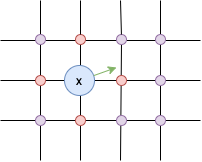
\includegraphics[scale=0.8]{gradient_example}
\caption{An example of how the gradient of a discrete state $x$ can be leveraged to pick the next state in 2
dimensional space. In this case, the gradient (green arrow) strongly points to the neighbour on the right side
of $x$ and slightly to the top neighbour. Based on this, we expect our method to choose the right neighbour as the
next state with a very high probability, while the top neighbour should be picked with the significantly less
probability and other neighbours should be ignored (neighbours are marked in red). Other states that are not direct
neighbours of $x$ are marked in purple.}
\label{fig:gradient_example}
\end{figure}

Now, we will show how to derive the update rule for the image denoising problem.\ Recall that the Ising model
for our problem is defined by the potential function
$$
H(e_i) = \prod\limits_{(j, k) \in K} e^{\beta e_i(v_j)e_i(v_k)}
\prod\limits_{j \in V} \mathbbm{1}_{e_i(v_j) = \tilde{Z}(v_j)}(1 - \alpha) +
\mathbbm{1}_{e_i(v_j) \neq \tilde{Z}(v_j)}\alpha
$$
which may be transformed to the more general form
$$
H(x) = e^{x^T W x} = e^{\tilde{H}(x)}
$$
where $W$ is $n \times n$ matrix encoding the observation and coupling components of the potential function.\ In
this formulation, the goal is to find $argmax_x \tilde{H}(x) = x^T W x$.\ Taking the gradient of
$\tilde{H}(x)$ with respect to $x$, we get
$$
(\nabla \tilde{H}(x))_i = (2W x)_i = \sum_{i, j} W_{ij} x_j
$$
which enables us to sample a neighbour of $x$ according to the probability distribution
$softmax(|\nabla \tilde{H}(x)|)$.\ Interestingly, we may interpret this process as a one step of the
Metropolis-Hastings algorithm with the proposal distribution
$$
Q_x = softmax(|\nabla \tilde{H}(x)|)
$$
which implies that in order perform our gradient-based update rule, one may use already developed
\textit{Algorithm} \ref{alg:metropolis_hastings}.\ Furthermore, the developed proposal distribution is simple as
it only takes into account the spins of neighbours of the current state and its consistency with observation
$\tilde{Z}$.

\section{Efficient implementation for image denoising}\label{section:efficient_denoising}

While developed gradient-based method provides a way to find pixels that should be updated, the naive
implementation performs one step of the algorithm in the time complexity $\mathcal{O}(|V|)$,
where $|V|$ denotes the number of pixels of a given image.\ In contrast, the Gibbs
algorithm provides the time complexity $\mathcal{O}(1)$ of one step, which means that it can update
$\mathcal{O}(|V|)$ random pixels while our method would update only one pixel in the same time.\ This issue makes
our method not scalable for high-resolution images.\ In this section, we will show how to reduce the complexity
of our algorithm to $\mathcal{O}(1)$, making it robust to a large number of pixels.\newline

Let us assume that the simulated chain is in the state $x$ and we have constructed the proposal distribution
$Q_x$.\ Now, we sampled some neighbour $x'$ that differs from $x$ by exactly one value of the sampled pixel
$\tilde{v} \in V$.\ The key observation is that most of the elements of $Q_{x'}$ are equal to the corresponding
elements of $Q_x$.\ Specifically, $Q_{x'}$ can differ in only 5 places, including $\tilde{v} $ itself and its
4 neighbours.\ It follows that instead of constructing the whole vector $Q_{x'}$ from scratch, one may recompute
it in only $\mathcal{O}(1)$ places.\ Furthermore, as each pixel contains only 4 neighbours, their potentials
can be updated in the time complexity $\mathcal{O}(1)$, which implies that the whole update step has the time
complexity $\mathcal{O}(1)$.\newline

The only part that still slows down our algorithm is the sampling step.\ Actually, the naive implementation of this
step has $\mathcal{O}(|Q_x|)$ time complexity, where $|Q_x| = |V|$.\ In order to reduce it, one may
observe that $Q_x$ is constructed in a way that it can take only $\mathcal{O}(1)$ values.\ Particularly,
for the binary image denoising problem there are $5$ possible values in the coupling part and $2$ possible
values in the observation part of the expression, which gives only $5 \cdot 2 = 10$ possible values.\ While in the
grayscale image denoising problem there are more possibilities, it can be significantly reduced by e.g.\ rounding
values in $Q_x$ to the nearest integers or ignoring very small values that are not likely to be drawn.\ In
practice, our experiments in \textit{Chapter} \ref{chapter:grayscale_experiments} show that such
approximations do not impact the quality of denoising, while they provide a significant improvement in terms of
execution time.\newline

As it is now clear that $Q_x$ can take only $\mathcal{O}(1)$ values, we provide \textit{Algorithm}
\ref{alg:sampling_from_q} for sampling from $Q_x$ as well as \textit{Algorithm} \ref{alg:updating_q} for
updating a potential of a specific pixel (neighbour).\ Both algorithms have the time complexity
$\mathcal{O}(1)$, implying that the whole step of the Metropolis-Hastings algorithm has the time
complexity $\mathcal{O}(1)$.\newline

\begin{algorithm}[H]
\caption{Sampling from $Q_x$}\label{alg:sampling_from_q}
\begin{algorithmic}[1]
\State{\textbf{Input:} A dictionary $P$ mapping potentials to pixels that have a custom potential}
\State{Compute the probability distribution $X$ over potentials utilising the information about the number
of elements on each list in $P$}
\State{Draw a list $L$ from the probability distribution $X$}
\State{Draw a pixel $p$ uniformly from the list $L$}
\State{\textbf{Output:} pixel $p$}
\end{algorithmic}
\end{algorithm}

\begin{algorithm}[H]
\caption{Updating a potential in $Q_x$}\label{alg:updating_q}
\begin{algorithmic}[1]
\State{\textbf{Input:} A dictionary $P$ mapping potentials to pixels that have a custom potential}
\State{\textbf{Input:} A dictionary $D$ mapping pixels to their potentials and positions on lists in $P$}
\State{\textbf{Input:} The position $p$ of a pixel and its new potential $v$}
\If{$p \in D$}
  \State{Find a list $L$ and a position of $p$ in $L$ by fetching this information from $D$}
  \State{Swap element $p$ from $L$ with the last element $e$}
  \State{Pop the last element from the list $L$}
  \State{Update the information about the position of $e$ contained in $D$}
\EndIf
\State{Update $P$ by adding $p$ to the end of the list $\tilde{L}$ corresponding to $v$}
\State{Update $D$ by providing $v$ and the position of $p$ in $\tilde{L}$}
\end{algorithmic}
\end{algorithm}

\numberedchapter{Experiments: binary images}

In this chapter, we will present the results of our experiments on binary images.\ In particular, we will compare
the developed gradient-based sampling method with the Gibbs sampling method.\ We will also explore how both methods
scale for high-resolution images and different noise levels.\ Lastly, we will show that our method
generates high-quality images even if the observation strength is not equal to the ground-truth noise level.

\section{Methodology}

In order to conduct experiments, we developed a binary images generator.\ Specifically, the generator produces
images by putting random geometric shapes on an initially empty image.\ To make the generated examples more complex,
except generating simple geometric figures, we also generate random text and lines.\ Some examples of
generated images along with their noisy versions are shown in \textit{Figure}
\ref{fig:binary_data_examples}.\ The images are generated in $300{\times}300$ and $1000{\times}1000$
resolutions.\ The noise is added by flipping random pixels, specifically each pixel is flipped with the probability
$\tilde{\alpha} \in \{0.05, 0.1, 0.15, 0.2\}$.\newline

In all experiments presented in the below sections, we sample 30 random binary images
(that meet given constraints).\ Then, we run the Gibbs sampling method and our gradient-based method for a
fixed number of iterations.\ During the optimization process, we measure the similarity between the currently
generated image and the ground-truth image by measuring the mean absolute error between the images:
$$
L_1(\tilde{X}, X) = \sum\limits_{i = 1}^n \frac{|\tilde{X}_i - X_i|}{n}
$$
where $\tilde{X}$ denotes the generated image and $X$ denotes the original image.\ As we keep pixel values in the
range $[0, 255]$, we have $L_1(\tilde{X}, X) \in [0, 255]$, where $0$ means that images are the same, while
$255$ means that all pixels are flipped.\ After running the optimization process for all considered images, the
$L_1$ errors are averaged.

\begin{figure}[H]
\centering
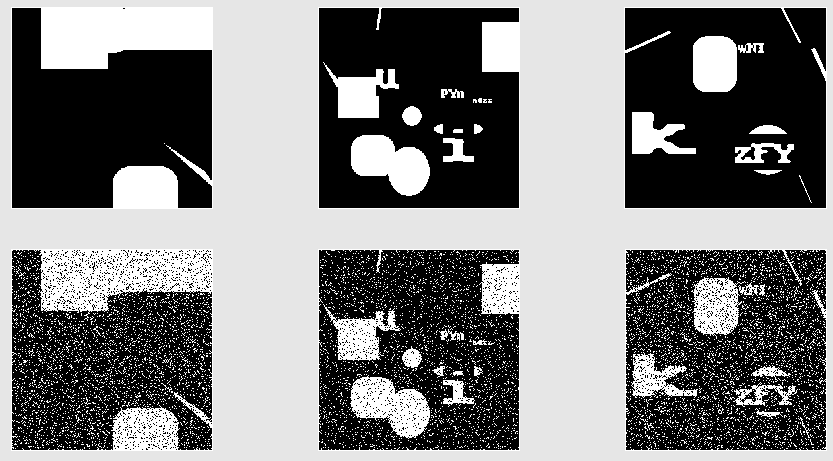
\includegraphics[scale=0.5]{binary_data_examples}
\caption{Examples of generated image pairs: ground-truth images (at the top) and observations (at the bottom).
The images on the left and in the center were generated with the noise level $\tilde{\alpha} = 0.1$, while the
image on right was generated with the noise level $\tilde{\alpha} = 0.15$.}
\label{fig:binary_data_examples}
\end{figure}

\section{Denoising quality based on image size}

As part of our analysis, we have plotted the rate of convergence depending on the input resolution.\ The
results of the experiment are shown in \textit{Figure} \ref{fig:binary_input_size_plots}.\ In
both cases of $300{\times}300$ and $1000{\times}1000$ images, the noise level was set to $\tilde{\alpha} = 0.1$
and the observation strength was set to $1 - \alpha = 1 - \tilde{\alpha}$.\ As it is shown in the plots,
the gradient-based method converges to an original image within an optimal number of steps.\ In contrast,
the Gibbs sampling method needs millions of iterations in order to converge to an original image.

\section{Denoising quality based on noise level}

In this section, we explore the impact of the noise level $\tilde{\alpha}$.\ In order to determine whether both
methods are able to reconstruct original images, we have run our experiments for
$\tilde{\alpha} \in \{0.05, 0.10, 0.15\}$ and set the observation strength $1 - \alpha = 1 - \tilde{\alpha}$.\ The
results of the analysis are shown in \textit{Figure} \ref{fig:binary_noise_level_plots}.\ From the presented
plots, it follows that both methods converge to the original images, even in the case of relatively high noise level.

\begin{figure}[H]
\centering
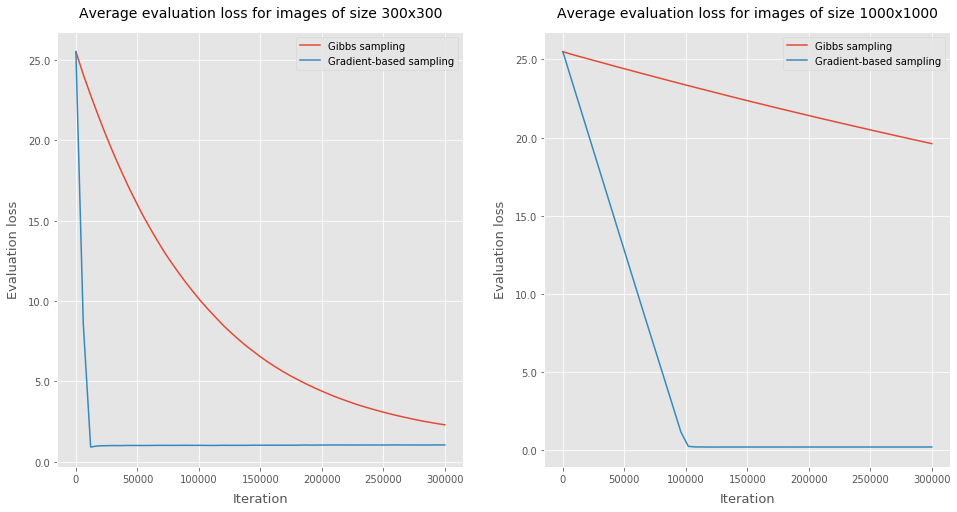
\includegraphics[scale=0.42]{binary_input_size_plots}
\caption{Comparison of the Gibbs sampling and our gradient-based method, based on input image size. The results
show that while the Gibbs algorithm needs millions of iterations in order to converge for $1000{\times}1000$ images, our
gradient-based method converges after roughly $100\ 000$ iterations.}
\label{fig:binary_input_size_plots}
\end{figure}

\begin{figure}[H]
\centering
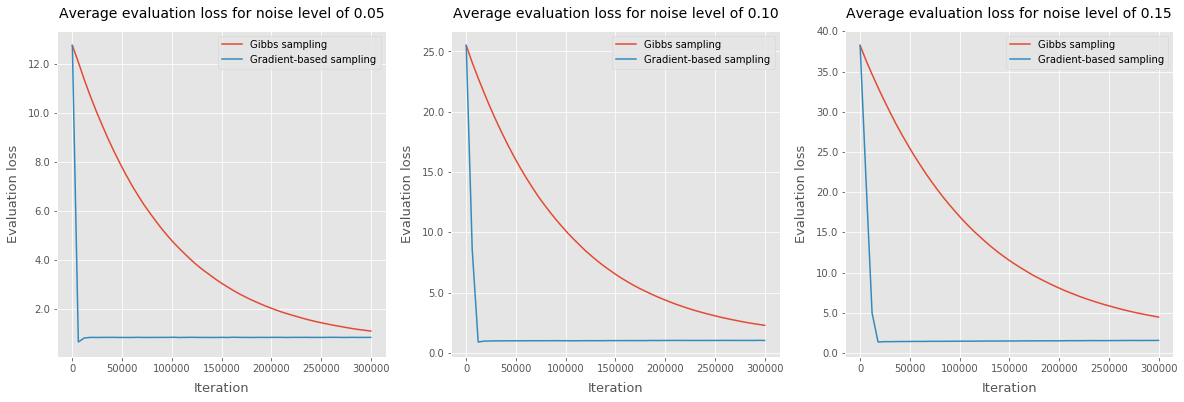
\includegraphics[scale=0.35]{binary_noise_level_plots}
\caption{Comparison of the Gibbs sampling and our gradient-based method, based on the noise level
$\tilde{\alpha}$. Both methods converge to the original images, regardless of the value of
the parameter $\tilde{\alpha}$.}
\label{fig:binary_noise_level_plots}
\end{figure}


\section{Sensitivity of the observation strength parameter}

In the previous sections, we leveraged the fact that the noise level $\tilde{\alpha}$ is known, by setting
the observation strength $1 - \alpha = 1 - \tilde{\alpha}$.\ In practical applications, it is often the case that
we observe an image without any hint how many pixels are flipped.\ In the present section,
we test different values of $\alpha \in \{0.01, 0.05, 0.15, 0.25, 0.35\}$, while keeping the value of the
noise level $\tilde{\alpha} = 0.05$ fixed.\ The results of our analysis are presented in
\textit{Figure} \ref{fig:binary_noise_level_prior_plots}, showing that our method estimates the original
image correctly even when the difference $|\alpha - \tilde{\alpha}|$ is high.

\begin{figure}[H]
\centering
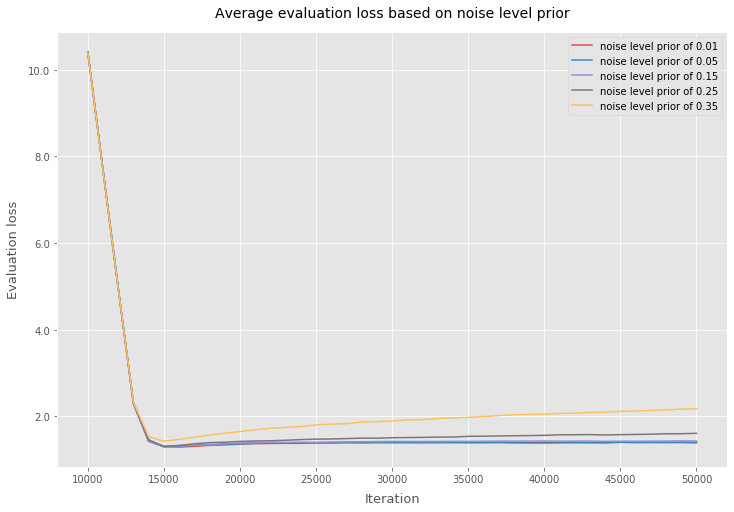
\includegraphics[scale=0.55]{binary_noise_level_prior_plots}
\caption{Comparison of the image reconstruction quality based on the observation strength $1 - \alpha$ for the
fixed noise level $\tilde{\alpha} = 0.05$. The $L_1$ errors are close $0.0$ in all cases expect for the cases of
$\alpha = 0.25$ and $\alpha = 0.35$ for which the errors are a bit higher, but still close to $0.0$. Interestingly,
in these two cases the quality degrades over time, suggesting that the optimization method has too
much flexibility.}
\label{fig:binary_noise_level_prior_plots}
\end{figure}

\section{Qualitative results}

The last conducted experiment involved comparing visual outputs produced by the Gibbs sampling and our
gradient-based method.\ To do so, we performed $100\ 000$ steps of both methods and converted the last states
of the simulated chains into images.\ The outcomes of this analysis are presented in \textit{Figure}
\ref{fig:binary_qualitative_results}.\ The results of this experiment confirms that our method is superior to
the Gibbs sampling method.\ In particular, our method generated images that look identical to the original images,
even in dense text areas.\ Furthermore, the difference of quality between both methods is more visible for
high-resolution images as our method scales better to high-dimensional data than the Gibbs sampling method.

\begin{figure}[H]
\centering
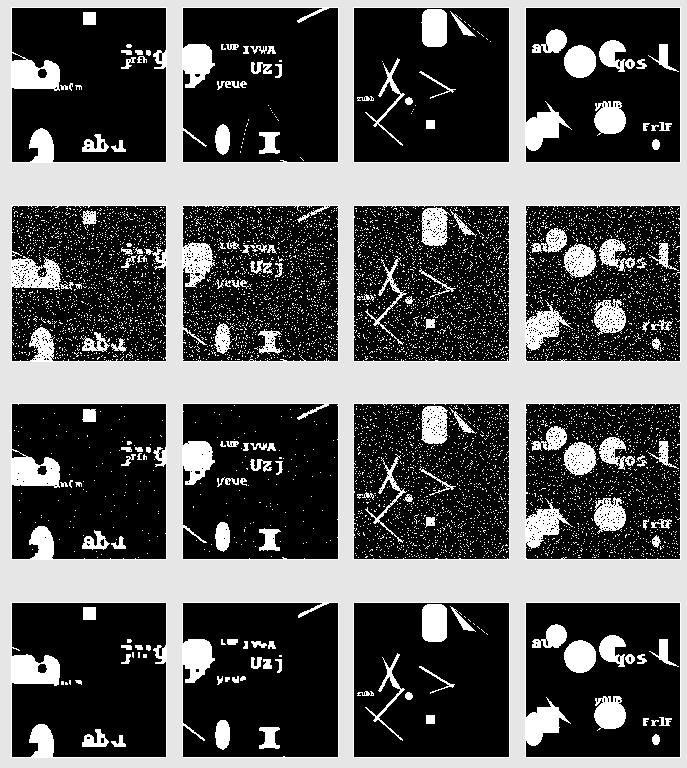
\includegraphics[scale=0.52]{binary_qualitative_results}
\caption{The comparison of the results generated by performing $100\ 000$ iterations of the discussed optimization
methods: original images (1st row), observed images (2nd row), images generated by the Gibbs
sampling method (3rd row) and our gradient-based method (4th row). While the images generated the Gibbs sampling
method contain quite a few noise pixels, our gradient-based method reconstructed the original images almost
perfectly. The images on the left side have a resolution of $300{\times}300$, while the images on the right side
have a resolution of $1000{\times}1000$.}
\label{fig:binary_qualitative_results}
\end{figure}

\numberedchapter{Experiments: grayscale images}\label{chapter:grayscale_experiments}

The problem of denoising grayscale images is more complex than the same problem for binary
images.\ Actually, the space of possible states is exponentially larger as each pixel can take $255$ different
values.\ In this chapter we will consider a model in which the noise is added to an original image by flipping
the values of random pixels.\ We will show that our method solves the stated problem in an effective manner
and present the results obtained on real photos.

\section{Methodology}

To run our experiments, we have collected $20$ grayscale photos and rescaled them to the fixed width of $800$,
keeping width-to-height aspect ratio of an original image.\ Then, for each photo we generated an
observation $Z$ by applying
$$
Z_{ij} =
\begin{cases}
  255 - X_{ij} &\text{if $U \sim Unif(0, 1) < \tilde{\alpha}$}\\
  X_{ij} &\text{otherwise}
\end{cases}
$$
where $\tilde{\alpha} \in \{0.1, 0.2\}$ controls the noise level.\ An example of an original photo along with
its noisy versions is presented in \textit{Figure} \ref{fig:grayscale_data_examples}.\ In order to
measure the quality of reconstructed images, we use already defined $L_1$ loss function
$$
L_1(\tilde{X}, X) = \sum\limits_{i = 1}^n \frac{|\tilde{X}_i - X_i|}{n}
$$
where $\tilde{X_i}, X_i \in \{0, 1,  \dots, 255\}$.\ The reconstruction errors are computed for all considered
photos and then averaged to obtain evaluation loss.

\begin{figure}[H]
\centering
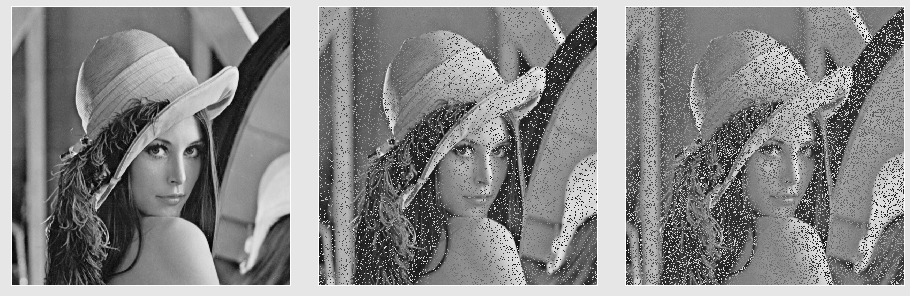
\includegraphics[scale=0.46]{grayscale_data_examples}
\caption{An example of real photo (on the left), the photo with the noise level $\tilde{\alpha} = 0.1$
(in the center), the photo with the noise level $\tilde{\alpha} = 0.2$ (on the right).}
\label{fig:grayscale_data_examples}
\end{figure}

\section{Denoising quality}

In order to determine whether our method is able to reconstruct original images, we performed the analysis with
$\tilde{\alpha} = 0.1$ and $\tilde{\alpha} = 0.2$ while comparing it with the Gibbs sampling method.\ We set
the observation strength $\alpha = \tilde{\alpha}$, however we observed that both optimization methods are not
sensitive to the value of this parameter and provide good estimations when $\alpha \neq \tilde{\alpha}$.\ The
results of our experiment are shown in \textit{Figure} \ref{fig:grayscale_noise_level_plots}.\ The first outcome
is that our method converges to an original image in an optimal number of steps, fixing some corrupted pixel in each
iteration.\ Furthermore, the errors are close $0.0$, meaning that the estimations of our method are near
perfect.\ Lastly, the Gibbs sampling method also converges to an original image, but it needs several million
iterations to provide a good estimation.

\begin{figure}[H]
\centering
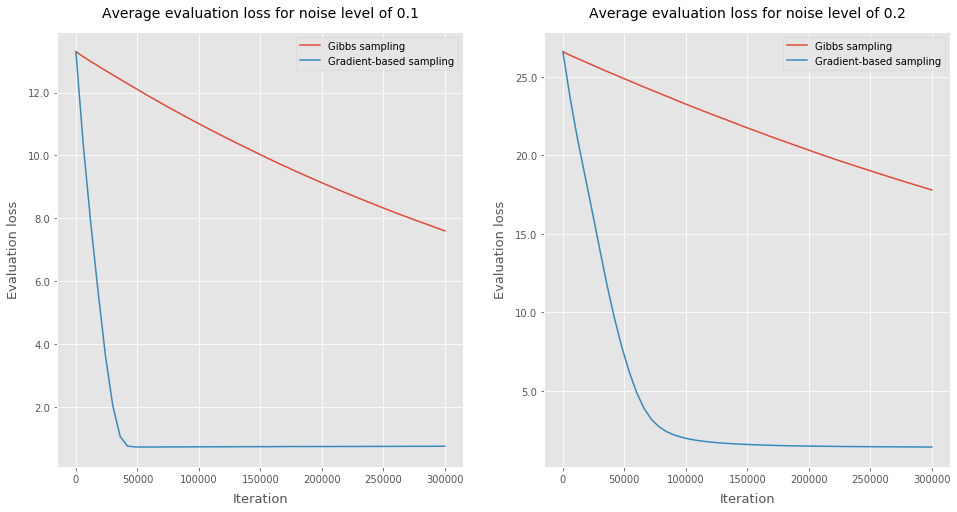
\includegraphics[scale=0.44]{grayscale_noise_level_plots}
\caption{Comparison of the Gibbs sampling and our gradient-based method, based on the noise level
$\tilde{\alpha}$. The results show that while both methods converge to the original images, our method generates
near-perfect estimation of an original image in relatively small number of steps}
\label{fig:grayscale_noise_level_plots}
\end{figure}

\section{Qualitative results}

In this section we present the visual comparison of images generated by the Gibbs sampler and our method.\ Like
in the case of binary images, we performed $100\ 000$ iterations of the discussed methods and converted the last
simulated states into images.\ The results of this analysis are shown in \textit{Figure}
\ref{fig:grayscale_qualitative_results}, proving that our method is able to reconstruct images in relatively
small number of steps.\ Particularly, our method reconstructed all $20$ images almost perfectly, while the
results generated by the Gibbs sampler were very noisy.

\begin{figure}[H]
\centering
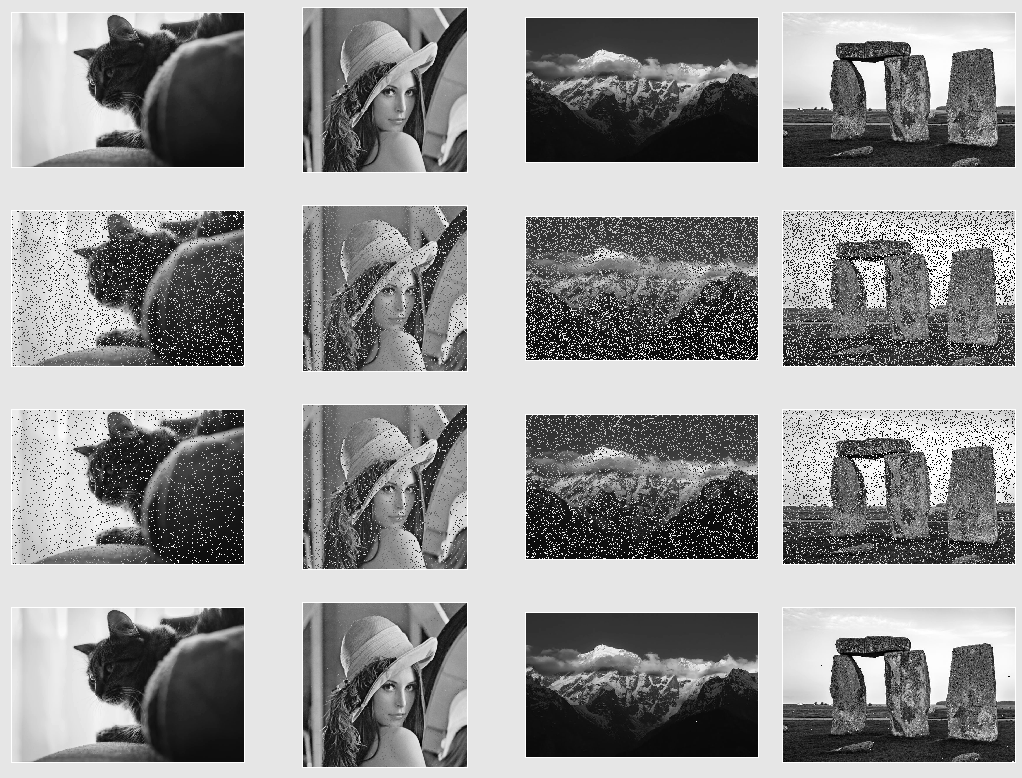
\includegraphics[scale=0.42]{grayscale_qualitative_results}
\caption{The comparison of the results generated after $100\ 000$ iterations of the discussed image denoising
methods: original images (1st row), observed images (2nd row), images generated by the Gibbs
sampling method (3rd row) and our gradient-based method (4th row). While the results obtained with the Gibbs
sampling method are very noisy, our reconstruction method generated images with hardly any corrupted pixels. The
images on the left side were generated with the noise level $\tilde{\alpha} = 0.1$, while the images on the right
side were generated with the noise level $\tilde{\alpha} = 0.2$.}
\label{fig:grayscale_qualitative_results}
\end{figure}

\numberedchapter{Summary}

TODO


\begin{thebibliography}{9}

\bibitem{markov_chains_book}
O. Häggström - \textit{Finite Markov chains and algorithmic applications (2002)}

\bibitem{mcmc_book}
P. Bremaud - \textit{Markov Chains: Gibbs Fields, Monte Carlo Simulation, and Queues (1999)}

\bibitem{oops_gradient}
W. Grathwohl, K. Swersky, M. Hashemi, D. Duvenaud, C. Maddison -
\textit{Oops I Took A Gradient: Scalable Sampling for Discrete Distributions (2021)}

\end{thebibliography}

\end{document}
